%===================================== CHAPTER 8 Implementation =================================

\chapter{Implementation}

This chapter discusses the details of the system implementation process, both for front-end and back-end implementation, but also how the project was managed throughout the process.


\section{Project progression}
The project progression derives from the product backlog (\textbf{Appendix \ref{app:product_backlog}}), meeting minutes (\textbf{Appendix \ref{app:meetingreport}}) and Trello archive and will only briefly summarize what was done at each sprint and only serves as a "quick tour" through the development process.

\begin{description}
	
	\item[Sprint 1 - 23.01.15 - 30.01.15] \hfill \\ 
	The first week mainly consisted of getting familiar with each other and the assignment. As soon as the introductions were done, we talked about our personal goals to set the expectation as a group. We formalized the rules of engagement (\textbf{Appendix \ref{app:rules_of_engagement}}) for the group to sign, and also delegated responsibilities. Later we established a meeting agenda with the customer and met with them for the first time.
	
	\item[Sprint 2 - 30.01.15 - 06.02.15] \hfill \\ 
	In sprint 2 we began planning and formalizing the requirements. Large sections of work like sketching a WBS (\textbf{Figure \ref{Fig:wbs}}), generating a product backlog (\textbf{Appendix \ref{app:product_backlog}}), and making use cases were done this week. Other design work like the architecture and UI mock-ups were also started on.
	
	\item[Sprint 3 - 06.02.15 - 13.02.15] \hfill \\ 
	This was the first week of development. We started testing the API (\textbf{Subsection \ref{subsec:back_end_tools}}) and finalized paper prototypes for user testing (\textbf{Subsection \ref{subsec:prototype}}) and also completed the design for the database and overall system architecture (\textbf{Figure \ref{Fig:architecture}} and \textbf{Figure \ref{Fig:er_diagram}}). Research on personalization (\textbf{Section \ref{sec:personalization_algorithms}}), the front-end framework Ionic (\textbf{Section \ref{subsec:ionic}}), and differences between the two operating systems \todo{ref crossplatform OS}IOS and Android were noted.
	
	\item[Sprint 4 - 13.02.15 - 20.02.15] \hfill \\ 
	For this sprint we analyzed the existing work done in the past (\textbf {Section \ref{subsec:stedr}}) to see if would fit our needs, and continued the research on collaborative filtering (\textbf {Section \ref{sec:personalization_algorithms}}). Some group members also spent time learning Docker (\textbf {Subsection \ref{subsec:docker}}). We mapped the Digitalt fortalt categories to our own (\textbf{Section \ref{sec:categorymapping}}) and conducted and evaluated the paper prototype tests as well. During this sprint the database code was also starting to take shape. We did a prioritization of the functional requirements in order to better plan the next sprint.  
	
	\item[Sprint 5 - 20.02.15 - 27.02.15] \hfill \\ 
	In this sprint we managed to get the harvesting (\textbf {Section \ref{sec:harvesting}}) up and running after the database was ready. A lot of work with the internal models on the back-end was done. The front-end team moved steadily though the initial work on the prioritized views (login, story and list). There was also a revision of the prototype to accommodate the customer's feedback from their user tests.
		
	\item[Sprint 6 - 27.02.15 - 06.03.15] \hfill \\ 
	Finalizing the database communication was done in order to fully test the front-end and to get the back-end team started on the personalization. The test plan (\textbf {Section \ref*{chap:testing}}) was in the stage of being attuned and formalized for the documentation. After the new prototype was finished, another round of user tests were conducted and the work continued on each of the application views.
	
	\item[Sprint 7 - 06.03.15 - 13.03.15] \hfill \\ 
	Some work to meet a report delivery was done early in the sprint. Later in the sprint, the back-end was showing good progress on finding/testing a suitable filtering framework, while the front-end refined the appearance of each view to better fit the user needs. The was also work done on resolving some issues with the server communication.
	
	\item[Sprint 8 - 13.03.15 - 20.03.15] \hfill \\ 
	The application was taking shape on many fronts, so this week we worked more on video support and started with the on-boarding section of the application. On the back-end the Mahout (\textbf {Section \ref{sec:personalization_how}}) framework setup was on the way. There was also some work spent on testing.

	\item[Sprint 9 - 20.03.15 - 27.03.15] \hfill \\ 
	This week we polished some features and functionality to hit the milestone Beta version (\textbf {Section \ref{sec:milestone_plan}}) in order to prepare the application for some testing in the wild during the upcoming Easter. Further development on the Mahout framework, content-based filtering and fixing of some unforeseen issues on the harvester was also done.
	
	\item[Easter - 27.03.15 - 07.04.15] \hfill \\ 
	The application was tested under informal conditions on family and friends, a so-called "in the wild" test.
	
	\item[Sprint 10 - 08.04.15 - 17.04.15] \hfill \\ 
	We dealt with the feedback from usability tests conducted during the Easter. Some platform-specific issues needed some focus to be resolved. We did some more polish on the views and cleared out some front-end bugs. on the back-end, work continued on both collaborative and content-based filtering, which it would for the rest of the sprints. 
	
	\item[Sprint 11 - 17.04.15 - 24.04.15] \hfill \\ 
	The application is nearly finished on a functional level. Resources were dedicated to polishing, and bug fixing became the focus while a lot of testing was conducted on the server. The last big task that the back-end worked on was to finalize the filtering.
	
	\item[Sprint 12 - 24.04.15 - 01.05.15] \hfill \\ 
	Sprint 12 was similar to sprint 11, but there was a significant increase in the workload this week due to the upcoming final milestone of having an application ready for delivery to the customer. We intended to accomplish this by the end of this week. This did not happen, but we had aimed for a final build earlier than necessary. We planned for some last minute changes and allowed time to fix undiscovered bugs, which was exactly what happened. We also used some extra time for unit and system testing.
	
	\item[Sprint 13 - 01.05.15 - 08.05.15] \hfill \\ 
	This week was spent on various bug fixing for some members of the group, while the majority did mainly report and documentation work. We planned an acceptance test with the customer the following week. We went through the application and did extensive functional testing prior to the customer meeting.
	
	\item[Sprint 14 - 08.05.15 - 15.05.15] \hfill \\ 
	During the testing done the week before, more undiscovered issues were uncovered and we needed some more time for polishing and fixing. We had not yet locked in a date for the customer to do an acceptance test, except before the end of the month. The customer agreed to set up a final meeting the following Monday, which we felt would give us time to take care of our main issues, and even give us some time to go the extra mile.
	
	\item[Past 15.05.15] \hfill \\ 
	At the start of the week we met with the customer to go through the functionality in conjunction with the functional requirements to see if the customer also thought we hit our goal (See \textbf {Section \ref{sec:acceptance_test}}).\newline
	  
	Work was conducted after the last sprint(sprint 14) this was mainly fixing some bugs, finalizing the report and the application and source code handover. The final burn down of the work progression for all the sprints is shown below in \textbf {Figure \ref{Fig:burnDownAfter}}.
	
\end{description}

\begin{figure}[h!]
	\centering
	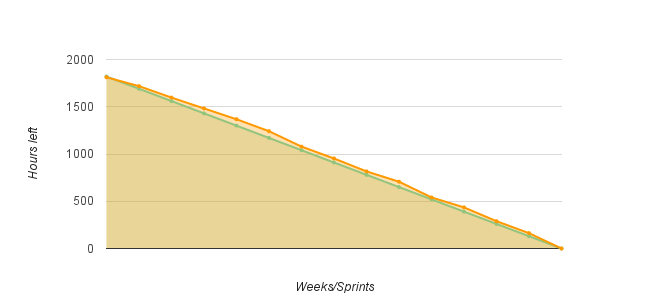
\includegraphics[width=\textwidth]{fig/burnDownAfter}
	\caption{Final burn down chart}
	\label{Fig:burnDownAfter}
\end{figure}

\section{Front-end}

This section will be an elaboration of some challenges and limitations that arose during the creation of the user interface, both concerning the design and the implementation aspects of the process.

\subsection{Designing the user interface}
\label{subsec:prototype}
The user interface design was an essential part of the project, as the customer prioritized usability over all other non-functional requirements. The design therefore went through many iterations of working on a prototype and continually getting feedback from customer and user tests. This feedback loop was important as the customer did not have all the specific requirements to the application from the beginning, and because making everything easy to understand for the user was also challenging. Balsamiq was first used to create a basic wireframe, but as its functionality was limited, the next iteration of the design was made using Proto.io. This made it possible to receive better feedback on the flow of the app and not just the views individually. \newline

While designing the user interface, some attention was paid to the projects described in \textbf{Section \ref{sec:existing_solutions}}. The group analyzed this previous work as a basis to decide what would be good or bad design choices for "Vettu hva?". A few general conclusions described in \textbf{Section \ref{sec:existing_solutions}} were that having static images occupying screen space is poor design, and that lists are normally easier to navigate than maps.\newline


The target audience for the application included both those who have an interest in cultural activities, and also those who do not have any interest or experience about this, so as to encourage more of the general population to discover an interest in the subject. A specific target audience of 16-19 year old teenagers were promoted as a possible focus, because of the possibility of encouraging a young audience to develop an interest in cultural heritage. However, this was not stated until around  midway in the project timeline. This fact made it difficult to consider target audience when making design decisions. \newline

The prototype has been through multiple iterations. Early on, it was imagined to have a sort of “magic” discovery function where a user would for example rub a crystal ball and receive a recommended story. This idea was later discarded because the team and customer realized
 it would be better usability to present the user with multiple recommended stories that they could simply browse through instead.\newline

Another of the early ideas was for the user to receive a “daily story” or some sort of schedule for being presented with recommended stories. However, due to workload and time constraints, this requirement was heavily down-prioritized. The most important parts were the personalization and usability aspects, so receiving notifications seemed like an unnecessary extra feature.\newline

In the first prototype a media preference view was also included when creating a new user. In this view the user should put the media formats (text, images, video, audio) in order by which format the user preferred. This was discarded in the second prototype, as it was difficult for users to understand the purpose of it and the customer agreed it was not necessary. 
\begin{figure}[h]
	\centering
	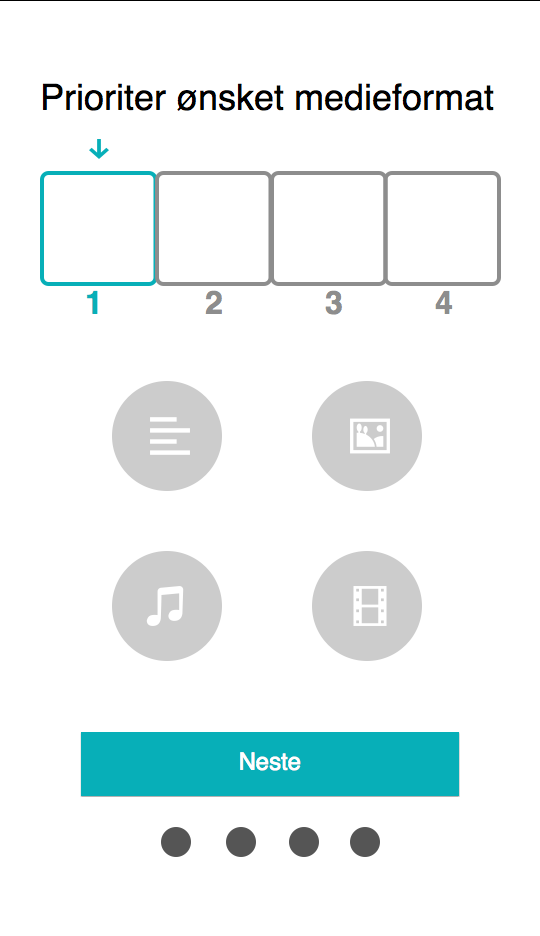
\includegraphics[scale=0.5]{fig/prototype_media}
	\caption{Media preference view from the first prototype which was later discarded.}	
\end{figure}

The application uses many different icons in various parts of the interface, and these have been the source of much debate and redesign. The icons used to represent categories were not always understood by users, and some categories like “local tradition and food” were difficult to represent universally with just a single icon. Also the bookmark icon shown in the upper right area of \textbf{Figure \ref{Fig:prototype}} was confusing to some users, and there was a concern in the team that this icon might not accurately represent that it allows the user to save the story in a bookmark list.\newline

A big issue for the interface design has been the handling of the different media elements (text, pictures, audio, video) and how these should be positioned relative to each other. For a while the team designed the application to have one tab for each of these four elements in the story view, as shown to the left in \textbf{Figure \ref{Fig:prototype}}. The customer had a concern that this might not be the optimal solution, as a user would for example not be able to read text and view pictures simultaneously. After some discussion, the interface was redesigned so that the text would be persistent, and instead the user could tab between pictures, audio, and video. The resulting design can be seen to the right in \textbf{Figure \ref{Fig:prototype}}. \newline

\begin{figure}
	\centering
	\begin{subfigure}[h]{0.3\textwidth}
		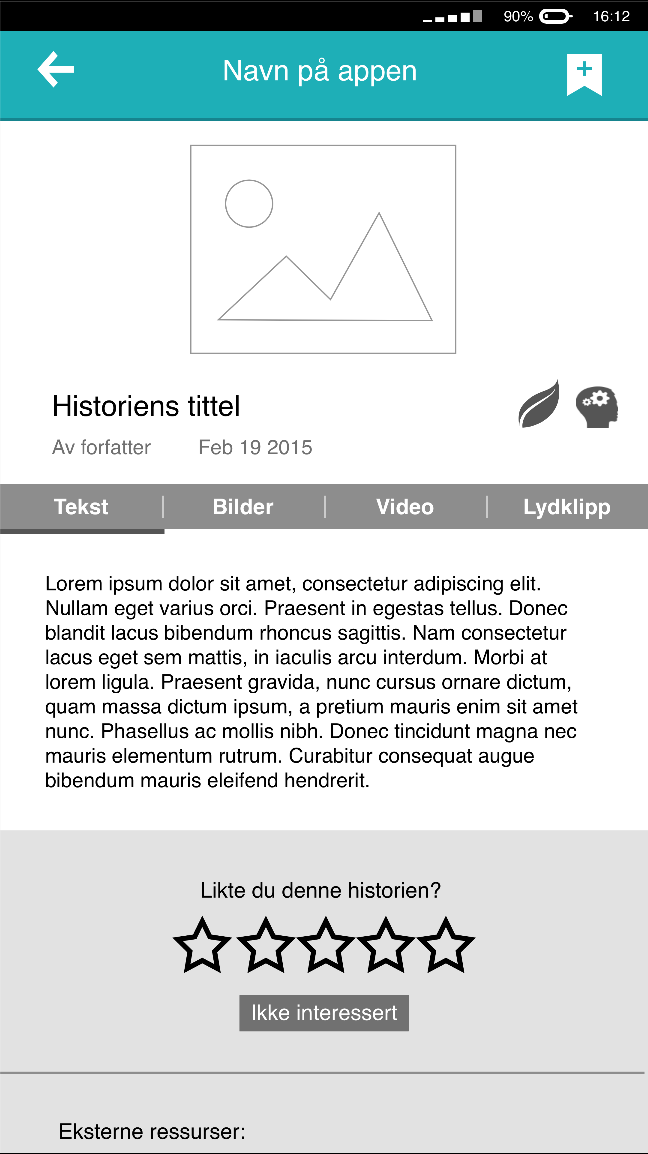
\includegraphics[width=\textwidth]{fig/prototype1}
	\end{subfigure}
	\begin{subfigure}[h]{0.3\textwidth}
		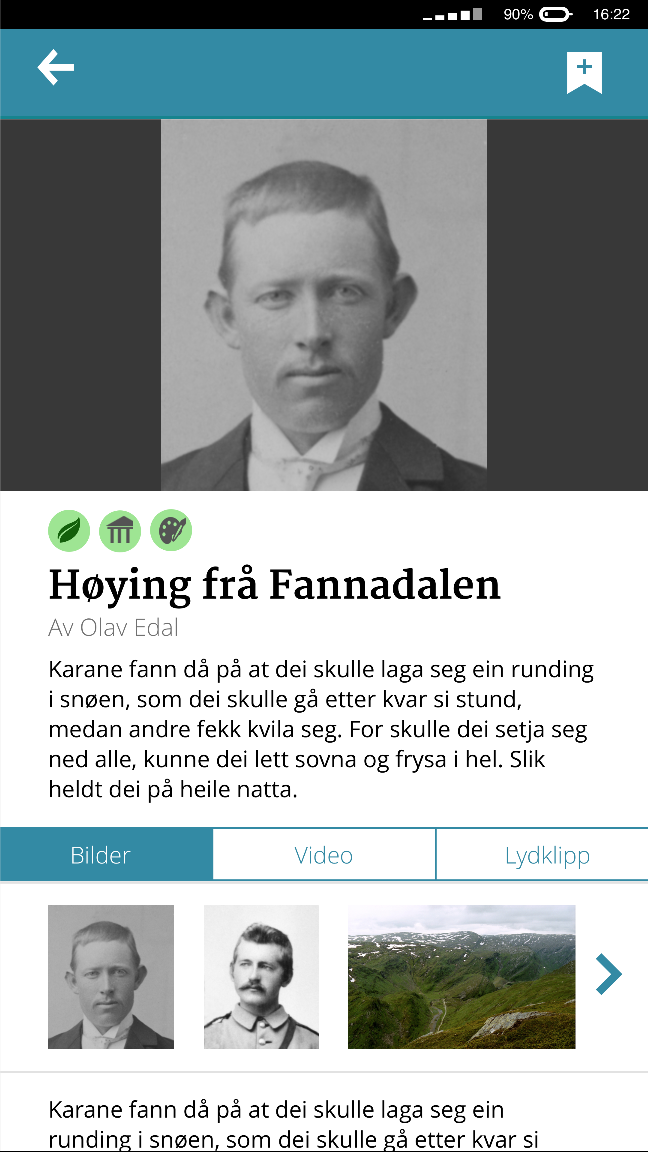
\includegraphics[width=\textwidth]{fig/prototype2}
	\end{subfigure}
	\begin{subfigure}[h]{0.3\textwidth}
		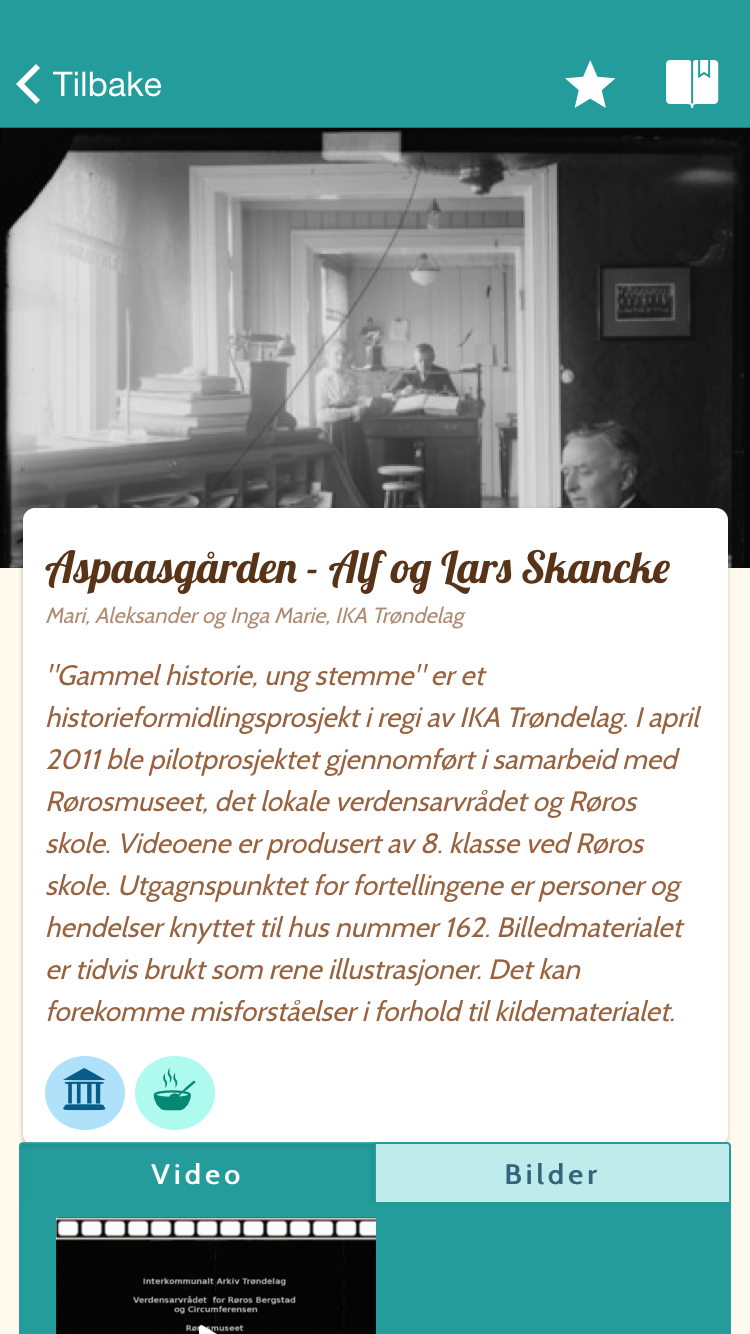
\includegraphics[width=\textwidth]{fig/screenshot_story}
	\end{subfigure}
	\caption{Comparison of the story view in the first and second versions of the prototype and the final design implemented.}
	\label{Fig:prototype}
\end{figure}


\subsection{Implementing the user interface}
\label{subsec:user_interface}

Early on in development, the team discovered several limitations to the Ionic framework. For example, when using a list to display stories, it was not possible to swipe the list both left and right. The idea was to swipe one way to add a story to be read later, and swipe the other way to reject a story from the list entirely.  Because this proved to be impossible, the views were redesigned into a different solution which was much less based around swiping.\newline

As this is an application for mobile devices, it had to be adapted to work on different screen sizes. The team found that it would most likely be best to target a relatively small screen size and then simply enlarge it for bigger screens. This eliminated the issue of having to compress the components to fit smaller screen sizes and potentially be forced to redesign the whole view to fit small screens.\newline


Adopting accurate naming conventions for the different components has also been a considerable issue. Stories can be saved in bookmark lists, but these lists have interchangeably been called collections and tags in the system. Also when asking a user to input their preferred categories to receive stories from, there has been some confusion because of interchangeably calling these categories for interests,  preferences, and categories.\newline

Implementing media, and especially video, has been a challenge in the project. An issue with this has been that playing videos is handled differently on iOS and Android, which had resulted in some bugs that only appear on one platform and not the other. These types of issues have been problematic to fix and has taken up much time. In addition, the videos provided by the Digitalt fortalt website come from different sources. Some of them are Youtube videos, others are Vimeo videos, and there are also other variations. Integrating all these different formats smoothly into the application has been a considerable challenge as well. \newline

Being able to reject a recommended story was a feature that was supposed to be implemented, but it was more difficult than it seemed. The problem was with the slide component from the Ionic framework, which did not do well with dynamic content. When removing a slide from the middle of the list of recommendations, it would not update properly and swiping did no longer work. \newline

It was also decided to remove the "not interested" option when rating a story. This was considered when testing the prototype, but was not decided until after the development had started. It was not intuitive what the button would actually do, and the user can convey the same "not interested" message in other ways. In order to rate, the user has to at least look at the story. If the user does not like the story after looking at it, then it is both more intuitive and useful that the user gives a low rating rather than "not interested". 





\section{Back-end}

This section describes the development of each part of the back-end. It aims to give a timeline of the development and explain how and why important decisions were made. The different parts described here are Docker, the database, the personalization, the choice of language and the e-mail part of the application.  

\subsection{Docker}

Using Docker as a deployment tool proved easier than initially expected. This is mainly because there exists a good amount of documentation and examples online. Initially the Docker setup was based entirely on a project called tutum \cite{EHW3}. Using this projects Dockerfile it is possible to only specify the Git repository of an application to have an Apache server running with this application. Furthermore, it is possible to define a password to use for the database. This suited the back-end work very well since it filled the initial requirements. However, as requirements developed and understanding of Docker increased, a more tailored and advanced setup was used. In this setup a second image is used to save the database between restarts, which means that it is possible to update code without having to start the database anew. In addition to this, harvesting from Digitalt fortalt is performed at 03:05 server time, each night. \\

Once work on personalization started it was necessary to have Java in the Docker image as well. This proved uncomplicated and worked as intended. Passwords and other important keys were put in a separate file that can be included along with the Dockerfile where this is required.

\subsection{Database}

Based on the first version of the functional requirements for the application, an initial ER-diagram was made in the middle of February. At this stage the customer and the team had not come to an agreement on a prioritization of the non-functional requirements. This meant that it was for instance not clear how important the performance of the system would be for the customer, an attribute of the system which would influence how much info should be stored for each story in the database versus how much info should be retrieved from Digitalt fortalt every time a user views a story. However, the changes to the initial diagram have been relatively minor. Some of the alterations were based on updated requirements from the customer (for instance regarding research data), while others stemmed from the group and were optimization of the data model or changes made to facilitate the personalization.\newline

The relational database was created from the ER-diagram using the mapping algorithm in \cite[p.270-278]{AS2}. Some of the tables in the database has the potential for NULL values, but this was accepted as it was considered more important to keep the mapping from one entity to one table. In addition, the database already had quite a few tables and further splitting would make the extraction of information more costly, with numerous join operations. \newline 

The team did not understand how to do the personalization until mid March. The decision on how to do this introduced changes to existing tables and the need to create additional tables and views in the database. Mahout had requirements for the input data, which meant that a view was created to store all the necessary data for collaborative filtering. Using this view made it straightforward to put the desired data from the database into Mahouts data model.

\subsection{Personalization}

At the start of the project much time was devoted to understanding content-based and collaborative filtering and how the theoretical descriptions of these techniques could be turned into a practical implementation in our application. When the back-end part of the group had a better understanding on how this could be done, an important decision was whether to use open-source recommender engines or to implement the algorithms ourselves. After studying the math and complexity involved in writing our own implementation it became clear that the best solution would be to use existing recommender engines, even if this would require some adjustments to already written code. \newline

As the project was nearly halfway through when the decision to use an open-source recommender engine was made, the team did not find the time to do a thorough review of the many different alternatives. This increased the probability of choosing the wrong tool to work with and violated the stated preventive action in the risk list (see \textbf{Appendix \ref{app:risklist}}). However, the customer suggested three different recommender engines that might be worth looking into, one of which was Mahout (see \textbf{Section \ref{sec:rec_tools}} for an evaluation of the three different engines). In choosing a tool the customer had done some research on, the group found that the risk of making a wrong choice decreased somewhat. In addition, Mahout presented its features in a way that resembled the groups research on filtering algorithms and it was therefore reason to believe that getting started with Mahout would not require much additional research. Of particular importance was the fact that Mahout offered a short explanation on how to do content-based filtering using their recommender engine. Most such engines provided functionality for doing collaborative filtering, but it was not always clear how content-based filtering could be done.\newline

Mahouts website provided some guiding on how to build a recommender which made it possible to use the tool without thorough knowledge of how the different methods worked. Most of the work in the beginning of doing the personalization thus centered around how to gather and produce data in a format acceptable to Mahout and how to treat the output recommendations. Content-based filtering was implemented first, as this was the customer's wish and because the first recommendations presented to a user would always be content-based. Since Mahout does not provide methods for finding similarities between items based on their attributes, the group had to implement this. There exist a vast number of functions to compute similarity between objects. The group did some research on different similarity measures, but the literature did not provide a clear-cut answer to which measure was best fitted to our data. Cosine similarity was chosen for its simplicity and because a story's subcategories lent itself well to be represented as a vector.\newline

The customer requested the use of both item-based and user-based collaborative filtering. There was some doubt in the group as to whether the produced recommendations from the two methods could be combined, but it was found that this was possible as both take the same data model as input. When doing user-based collaborative filtering, a threshold value had to be set to tell the recommender engine which users should affect the recommendations. This concerns the similarity found between users. It was difficult to set this value as the computation of the similarity is done by Mahout and because the group did not know what threshold value would be reasonable to set. The value is set by means of trial and error, looking at the resulting recommendations produced using different values, and by looking at example use of this method. \newline

A challenge in the project has been to assess the quality of the recommendations. Reasons for this has been the limited amount of harvested stories and the use of Mahout as a black box. The first point was a limitation set by the customer. They wanted to limit the amount of harvested stories to ease the evaluation of "Vettu hva?". With fewer stories the probability of different users reading the same stories would increase, and thus require fewer users to get the collaborative filtering running (the cold start problem described in \textbf{Section \ref{subsec:prestudy_collaborative}} would be resolved faster). \newline

The second point was down to the implementation of the project and mainly concerns collaborative filtering. Content-based filtering has fewer variables and it was possible to check if input categories produce recommended stories that in fact are connected to those categories. Collaborative filtering involves more variables and it was not obvious from the raw data to see which users should influence recommendations for a user and what weights to assign to the different users preference values. In general, collaborative filtering finds patterns in the data that are less obvious found there than content-based filtering. By using Mahout as a black box this pattern finding has been hidden to the team. This could have been remedied by studying the implementation of Mahout, but the time required to do this was not found to be within the confines of the project. A broader test of the application with real users could also have given some insight into the quality of the recommendations, but this was outside the scope of the project. \newline


\subsection{Language}
\label{subsec:backend_language}
\textbf{PHP}\newline
PHP is a server-side scripting language produced by The PHP Group that is especially suited for web development  \cite{HM8}. It is a general-purpose scripting language often used to provide dynamic content from a web server to a client. During the pre-study period several reasons for choosing PHP as the main back-end language were presented. Firstly, all back-end team members were experienced in the use of PHP. Secondly, as inexperienced users of Docker, more documentation existed on how to implement PHP with Docker than with the other language alternatives considered. Lastly, it was easily combined with the HTTP protocol used by front-end to request and receive data (see \textbf{Section \ref{subsec:frontend-backend_communication}}).\newline

\noindent\textbf{Java}\newline
Java is a very popular general-purpose object oriented programming language developed by Sun Microsystems and later Oracle Corporation \cite{HM9}. Java was later in the project chosen as a secondary back-end language. This was because Mahout, which was used to implement the recommender engine (see \textbf{Section \ref{sec:personalization_how}}), is written in Java. 


\subsection{E-mail}

To create a user in “Vettu hva?” the user only needs to provide an e-mail address. E-mail was chosen as the identifier because it is unique for a specific person. When a user tries to log in and the e-mail does not exist in the database, a new user is created and the user is assigned a user ID and the ID is returned to front-end. A message is also sent to the provided e-mail, to confirm that the user is registered. If the e-mail already exists, the previously created user ID is returned to front-end and the user can continue where he/she left of. The mail service used to send the confirmation e-mail is an e-mail sending library for PHP called PHPMailer. Originally, the plan was to use the built in mail() function in PHP. However, in order for this to work a properly configured local SMTP server was required. This proved to be too much work for this assignment, so the solution was to use PHPMailer with a “Vettu hva?” gmail. PHPMailer can be used to send e-mails from existing mail servers, like Google Mail, by providing a username (gmail) and password.

\cleardoublepage